\subsection{Singleton}

\textbf{Definición:} El patron singleton o de instancia única tiene el objetivo de restringir la creación de una clase a una sola instancia que pueda ser accedida de manera global. Este parón es quizás el mas sencillo debido a que no presenta un alto grado de complejidad y no requiere técnicas elaboradas de desarollo para llevar a cabo su implementación.

\textbf{Motivación:} En ocasiones necesitamos que una clase tenga exactamente una instancia, como por ejemplo para la definición de una instancia única base de datos, una variable de acceso global a una estructura de datos compleja o cuando nuestra aplicación realiza procesamiento de datos concurrentes que requieren acceder a un objeto de instancia común.

\textbf{¿Como puedo implementar un singleton?:} Para crear un singleton, deberíamos ser capaces de definir la estrutura necesaria para asegurar que un objeto de una clase cualquiera solo pueda ser instanciada una vez, una de las formas mas comunes de hacerlo es mediante un constructor privado que impida a clases externas realizar su instanciación y ocultar la lógica encargada de la instanciación del objeto dentro de un método público definido en la clase.

\textbf{Escenarios de aplicación:}

\begin{itemize}
	\item Debe existir exactamente una instancia de una clase y su acceso debe ser global
\end{itemize}

\textbf{Modelo UML:}

El aspecto mas importante de este patrón es la definición de un método privado que se encargue de la instanciación del objeto, lo cual garantiza que el objeto solo pueda ser creado una vez, así cuando un Cliente específico requiera utilizar el objeto solo deba preocuparse por obtener la instancia.

\begin{figure}[H]
	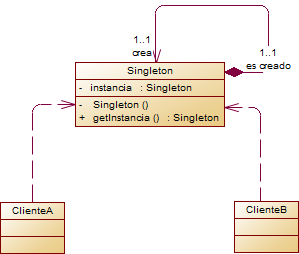
\includegraphics[width=0.7\textwidth]{images/creational/singleton/singleton.png}
\end{figure}

\textbf{Ejemplo conceptual:} De acuerdo a las teorías actuales aceptadas en cosmología, existe un unico Universo en el cual vivimos y existe todo lo que conocemos. Imaginemos el mecanismo que pudo llevarse a cabo para permitir que este Universo existiera, hasta donde sabemos solo existe una instancia de nuestro Universo y no hay pruebas concluyentes que indiquen la existencia de otros Universos. Por algún motivo fuera de nuestro entendimiento la naturaleza decidió que el Universo fuera un singleton. A continuación intentaremos abstraer la lógica necesaria para crear un Universo y plasmarlo en un programa computacional.

Inicialmente, se podría pensar en la creación de una clase \textbf{SingletonUniverso} que se encargue de implementar la lógica necesaria para crear y mantener una sola instancia del Universo durante toda la ejecución del programa. Para ello, se define un constructor privado \textbf{SingletonUniverso()} que impida a otros crear nuevas instancias.

\begin{figure}[H]
	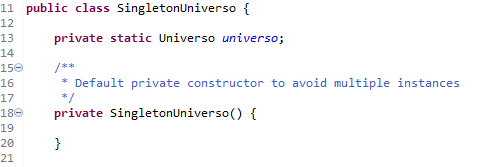
\includegraphics{images/creational/singleton/singletonExample1.png}
\end{figure}

Ya tenemos nuestro posible nuevo Universo, ahora es necesario implementar el mecanismo para que su instanciación sea única, el patrón singleton propone la creación de una función pública  \textbf{getInstancia()} que tendra cumplirá dos funciones: (i) crear una nueva instancia si no existe y (ii) retornar la instancia cuando esta ya exista. De manera opcional se pueden crear métodos adicionales que se encarguen de funciones específicas relacionadas al dominio de la aplicación.

\begin{figure}[H]
	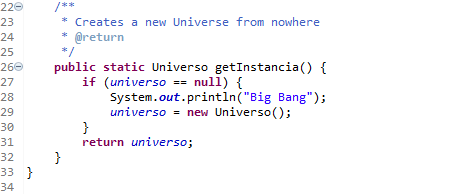
\includegraphics{images/creational/singleton/singletonExample2.png}
\end{figure}

Como se puede observar, la implementación del singleton no conlleva lógica adicional, una vez creada la definición general de la clase solo basta con que una clase externa requiera instanciar un Universo. De acuerdo a la forma en la cual fue definida la clase es imposible realizar su instanciación de manera directa, resultando en un error de compilación indicando que el constructor de la clase no es visible.

\begin{figure}[H]
	
\includegraphics{images/creational/singleton/singletonExample3.png}
\end{figure}

Por otro lado, el patron garantiza que solo exista un Universo en nuestra aplicación, un usuario todopoderoso que requiera crear un nuevo Universo está obligado a invocar el método \textbf{getInstancia()}, si por alguna razón necesita crear uno nuevo se encontrará con que es imposible gracias a que el diseño solo permite una única instancia.

\begin{figure}[H]
	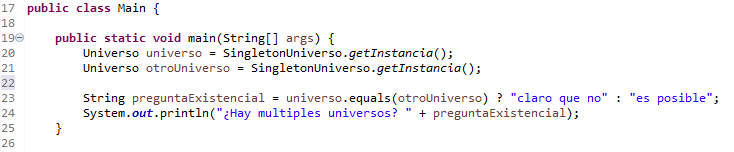
\includegraphics{images/creational/singleton/singletonExample4.png}
\end{figure}

Gracias a la flexibilidad ofrecida por los lenguajes orientados a objetos es posible identificar si dos instancias de una clase hacen referencia al mismo objeto, en particular, JAVA permite realizar una comparación con el método equals (que para este propósito es mas que suficiente), obteniendo que los dos Universos creados son en efecto el mismo, cumpliendo con el objetivo del patrón.

\begin{figure}[H]
	
\includegraphics{images/creational/singleton/singletonExample5.png}
\end{figure}

Un aspecto interesante del patrón singleton es que puede ser violado. Algunos lenguajes de programación como JAVA o C++ cuentan con librerías externas que permiten clonar una clase, acceder a las propiedades de clase a través de reflexión o deserializar de la clase, este tipo de operaciones permiten instanciar nuevos objetos saltando el control establecido por el singleton, lo cual viola el principio de unica instancia propuesta por el patrón. Existen diferentes técnicas que permiten evitar este comportamiento, por ejemplo lanzando una excepción en tiempo de ejecución que impida al usuario clonar el objeto o sobreescribir el método clone() para modificar su comportamiento.

Imaginemos un escenario en el cual un programador audaz decida de manera deliberada intentar clonar nuestro Universo implementando la interfaz \textbf{Cloneable}

\begin{figure}[H]
	
\includegraphics{images/creational/singleton/singletonExample6.png}
\end{figure}

Como resultado, nuestro amigo todopoderoso podría romper la regla de instancia única y crear múltiples Universos identicos al nuestro.

\begin{figure}[H]
	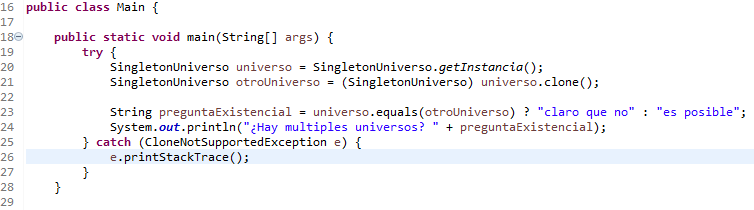
\includegraphics{images/creational/singleton/singletonExample7.png}
\end{figure}

Finalmente, el propósito del patrón se pierde

\begin{figure}[H]
	
\includegraphics{images/creational/singleton/singletonExample8.png}
\end{figure}

 Realizar este tipo de acciones no tiene sentido ya que destruyen el propósito del patrón. Por otro lado, es posible observar que la implementación comienza a volverse engorrosa porque obliga al desarrollador a validar escenarios adicionales de excepción, lo que limita el alcance de la solución y la vuelve menos flexible.

De manera análoga al caso anterior, el patrón podría ser violado mediante reflexión de clases u otros artilugios ingeniosos, sin embargo se debe tener presente que este no es el objetivo del patrón. Para evitar estos escenarios no deseados el desarrollador puede decidir agregar implementaciones adicionales al singleton que dote a la clase con los mecanismos necesarios para evitar estos comportamientos. Uno de los aspectos mas destacables en los esfuerzos por evitar esta situaciones se centra en realizar mejoras a los lenguajes de programación para evitar que se puedan realizar estas acciones, por ejemplo, a partir de la versión de Java 8 ya no es posible instanciar un singleton utlizando reflexión. Otros autores proponen apoyarse en el uso de estructuras como los Enumerados (o Enum) que limitan la creación de objetos. De acuerdo a Joshua Bloch en su libro "Java Best Practices", el uso de enumeradores permite facilitar la implementación de un Singleton y facilitar el trabajo de pruebas unitarias asociadas a la clase. Finalmente se debe tener siempre en cuenta que la decisión final de respetar la arquitectura es del desarrollador.